\renewcommand{\prevlecture}{11 }
\renewcommand{\thislecture}{12 }
\renewcommand{\nextlecture}{0 }

%
% Cover page
%

\title[PHYS 201 / Lecture \thislecture]
{
  PHYS 201 / Lecture \thislecture\\
  {\it Alternating Currents (AC); Resistor, Capacitor and Inductor in an AC circuit; The RLC series AC circuit}\\
}

\author[C.Andreopoulos] {
  Professor Costas Andreopoulos\inst{1,2}, {\it FHEA}
}
\institute[Liverpool/STFC-RAL] {
   \inst{1} University of Liverpool, Department of Physics\\
   \vspace{0.1cm}
   \inst{2} U.K. Research \& Innovation (UKRI), Science \& Technology Facilities Council,\\
            Rutherford Appleton Laboratory, Particle Physics Department\\
   \vspace{0.5cm}
   {\it {\color{magenta} Lectures delivered at the University of Liverpool, 2020-21}}\\
   \vspace{0.2cm}
}
\date{\today}

\titlegraphic{
  
\includegraphics[height=25px]{./images/logo/liverpool.png}
  \hspace{3px}
  
\includegraphics[height=30px]{./images/logo/ral.png}
}


\begin{frame}[plain]
  \titlepage
\end{frame}

% ------------------------------------------------------------------------------
% ------------------------------------------------------------------------------

%
% Revision of previous lecture
%

\renewcommand{\lecturesummarytitle}{Revision }

\renewcommand{\summarizedlecture}{11 }

%
%
%

\begin{frame}{Lecture \summarizedlecture - \lecturesummarytitle}

\begin{columns}
  \begin{column}{0.25\textwidth}
    \begin{center}
       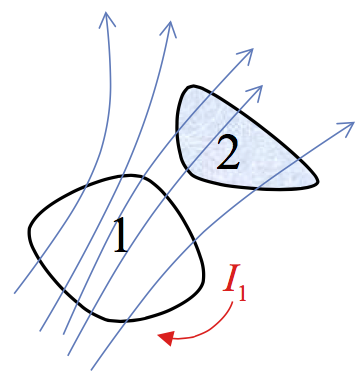
\includegraphics[width=0.90\textwidth]{./images/schematics/mutual_inductance_1.png}\\
     \end{center}
  \end{column}
  \begin{column}{0.75\textwidth}
  {\scriptsize
       The flux through the surface of loop 2, of the magnetic field $\vec{B}_1$
       produced by the current $I_1$ in loop 1 is:
       \begin{equation*}
            \Phi_2 = M_{21}  I_1
       \end{equation*}
       The constant of proportionality ($M_{21}$) is known as {\bf mutual inductance}.\\
       It is:
       \begin{itemize}
           \item purely geometrical, and
           \item unchanged if one switches the roles of loop 1 and 2.\\
       \end{itemize}
   }
  \end{column}
\end{columns}

\vspace{0.4cm}

{\scriptsize
       So \underline{whatever} the shapes and positions of the loops,
       the flux through loop 2 when we run a current I around loop 1 is
       identical to the flux through loop 1 when we run the same current around loop 2.
      \begin{equation*}
            M_{21}  = M_{12} = M
       \end{equation*}

        The SI unit of the mutual inductance is the {Henry} (H)
        \begin{itemize}
              \item A derived unit.
              \item 1 H = $\displaystyle \frac{Wb}{A}$ = $\displaystyle \frac{V \cdot s}{A}$
        \end{itemize}
}
\end{frame}

%
%
%

\begin{frame}{Lecture \summarizedlecture - \lecturesummarytitle (cont'd)}

{ \scriptsize
We also considered what happens if the current varies with time.
\begin{itemize}
  { \scriptsize
   \item  time-varying current $\rightarrow$ time-varying magnetic field
   \item  time-varying magnetic field $\rightarrow$  time-varying flux.
   \item  time-varying flux $\rightarrow$ EMF (Faraday's law)
  }
\end{itemize}

\vspace{0.3cm}

{\bf A change in current flow in a conductor induces a voltage (EMF)}
\vspace{0.2cm}
\begin{itemize}
  { \scriptsize
   \item in the same conductor (self-inductance): \\
             $\displaystyle \mathcal{E} = - L \frac{dI}{dt}$
   \vspace{0.2cm}
   \item and in neighbouring conductors (mutual inductance):\\
            $\displaystyle \mathcal{E}_{neighbouring\;loop} = - M \frac{dI}{dt}$
  }
\end{itemize}

\vspace{0.2cm}

In both cases the inductance (mutual or self) is the {\bf constant of proportionality}
between the EMF developed and the rate of current change.

\vspace{0.2cm}

We also studied the solenoid and its inductance per unit length (far from the ends of the solenoid) is:
\begin{equation*}
  L =  \mu_0 \cdot n^2 \cdot A
\end{equation*}
where $A$ is the area of each winding, and $n$ the number of turns per unit length.
}
\end{frame}

%
%
%

\begin{frame}{Lecture \summarizedlecture - \lecturesummarytitle (cont'd)}

Then we studied DC circuits with resistors, capacitors and inductors.

\begin{columns}
  \begin{column}{0.40\textwidth}
    \begin{center}
         \begin{circuitikz} [scale=0.7]
            \draw
                 (0,0) to[battery=$\varepsilon$] (0,2)
                         to[short, -o] (0.75, 2.0);
             \draw[very thick]
                  (0.78,2.0)--(1.22,2.0);
             \draw
                  (1.25, 2.0) to [short, o-] (2,2)
                                   to[R=$R$, i=$I$] (2,0)
                                   to[L=$L$] (0,0);
         \end{circuitikz}
     \end{center}
  \end{column}
  \begin{column}{0.60\textwidth}
   {\scriptsize
       We studied an RL circuit and we saw that its behaviour is determined
      by the following differential equation:
       \begin{equation*}
              \mathcal{E} -L \cdot \frac{dI}{dt} = I \cdot R
      \end{equation*}
   }
  \end{column}
\end{columns}

\begin{columns}
  \begin{column}{0.40\textwidth}
       \begin{center}
           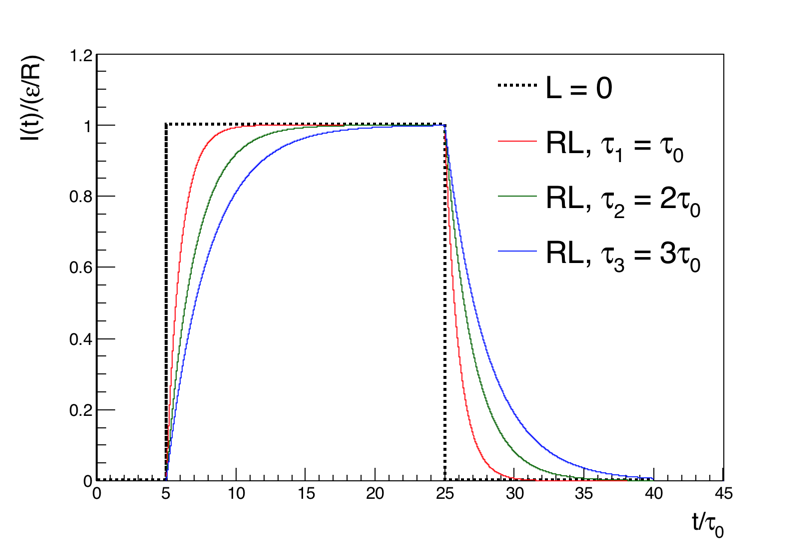
\includegraphics[width=0.95\textwidth]{./images/misc/ItRL_2.png}\\
       \end{center}
  \end{column}
  \begin{column}{0.60\textwidth}
  {\scriptsize
      We solved that equation which gave as the following solutions for the
      current after connecting or disconnecting the EMF:
      \begin{equation*}
       {\color{magenta}
            I(t) = \frac{\mathcal{E}}{R} \Big(1 - exp^{-\frac{t}{\tau}} \Big)
       }
       \;\;\; and \;\;\;
      {\color{magenta}
           I(t) = \frac{\mathcal{E}}{R} \cdot exp^{-\frac{t}{\tau}}
      }
      \end{equation*}
      Note that times are measured from the corresponding point of
      connecting or disconnecting the EMF.\\
  }
  \end{column}
\end{columns}

{\scriptsize
  {\bf Inductance is a kind of inertia in the circuit}. \\
  \vspace{0.1cm}
  So it is {\bf no longer possible to just change the current instantaneously} (as when L=0).
}
\end{frame}

%
%
%

\begin{frame}{Lecture \summarizedlecture - \lecturesummarytitle (cont'd)}

{ \scriptsize
We saw that the energy stored in the magnetic field of an inductor is: $\displaystyle U_B = \frac{1}{2} LI^2$.\\

\vspace{0.2cm}
Then we studied LC and RLC circuits both qualitatively and quantitatively:
\begin{columns}
  \begin{column}{0.50\textwidth}
     \begin{center}
         \begin{circuitikz} [scale=0.8]
            \draw
                 (0,0) to[battery=$\varepsilon$] (0,2) to[short, -o] (0.75, 2.0);
             \draw[very thick]
                  (0.78,2.0)--(1.18,2.3);
             \draw
                  (1.25, 2.0) to [short, o-] (2,2) to[C=$C$] (2,0)--(0,0);
              \draw
                  (2,2)--(4,2) to[L=$L$,i=$I$] (4,0) -- (2,0);
         \end{circuitikz}
     \end{center}
  \end{column}
  \begin{column}{0.50\textwidth}
     \begin{center}
         \begin{circuitikz} [scale=0.8]
            \draw
                 (0,0) to[battery=$\varepsilon$] (0,2) to[short, -o] (0.75, 2.0);
             \draw[very thick]
                  (0.78,2.0)--(1.18,2.3);
             \draw
                  (1.25, 2.0) to [short, o-] (2,2) to[C=$C$] (2,0)--(0,0);
              \draw
                  (2,2) to[R=$R$]  (4,2) to[L=$L$,i=$I$] (4,0) -- (2,0);
         \end{circuitikz}
     \end{center}
  \end{column}
\end{columns}

\vspace{0.2cm}

RL and RLC are described by the following differential equation (with R=0 for LC):
\begin{equation*}
          L \frac{d^2q}{dt^2} + R \frac{dq}{dt} + \frac{1}{C}q = 0
\end{equation*}

\vspace{0.2cm}
\begin{itemize}
\item
 Which saw that for R=0 we have undamped oscillations of charge, current and voltage and
that the stored energy is transferred fully between the capacitor (electric field) and the
inductor (magnetic field).
\item
For R$\ne$0 we have damped oscillations as, on every iteration, a fraction of the available energy is
converted to heat.
\end{itemize}
}

\end{frame}


%
% Plan for this lecture
%

\begin{frame}{Plan for Lecture \thislecture}

\begin{itemize}
\item Alternating Currents (AC)
\item AC generation: Simple alternator
\item Forced (or driven) oscillations
  \begin{itemize}
      \item Resistor (R) in an AC circuit
      \item Capacitor (C) in an AC circuit
      \item Inductor (L)  in an AC circuit
      \item The RLC series AC circuit
  \end{itemize}

\end{itemize}

\end{frame}

% ------------------------------------------------------------------------------
% ------------------------------------------------------------------------------

%
%
%

\begin{frame}{Alternating Currents (AC)}

So far we studied {\bf Direct Currents (DC)} meaning
\begin{itemize}
  \item voltage that maintains constant polarity over time, or
  \item current that maintains constant direction over time.
\end{itemize}

\vspace{0.4cm}

{\bf DC is the kind of electricity made by a solar cell or a battery}.\\

\vspace{0.2cm}

Other sources of electricity (most notably rotary electro-mechanical generators)
produce voltages that {\bf alternate their polarity} over time.\\

\vspace{0.4cm}

Either as a voltage switching polarity or as a current switching direction,
this kind of electricity is known as {\bf Alternating Current (AC)}.\\

\vspace{0.4cm}

{\bf AC is the kind of electricity that comes to your home}. \\
Typically in Europe we get a voltage of 220-240 V which alternates its polarity 50 times per second.

\end{frame}

%
%
%

\begin{frame}{Alternating Currents (AC)}

\begin{itemize}
  \item In some cases AC holds no practical advantage over DC.
     \begin{itemize}
        \item For example, in applications where electricity is used
                  to dissipate energy in the form of heat, the polarity or direction of current is irrelevant.
     \end{itemize}
  \vspace{0.3cm}
  \item However, with AC it is possible to build {\bf long-distance power
            distribution systems} that are far {\bf more efficient than DC}
     \begin{itemize}
         \item AC is used predominately across the world in high power applications.
     \end{itemize}
\end{itemize}

\begin{center}
    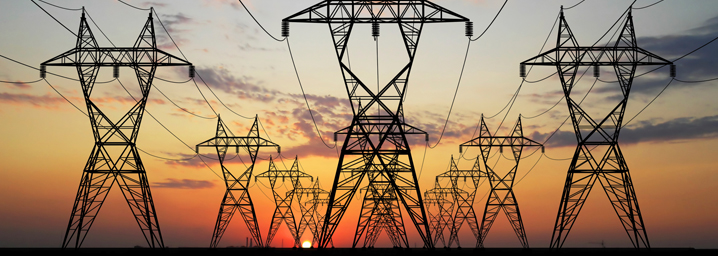
\includegraphics[width=0.70\textwidth]{./images/photos/power_distribution_01.jpg}\\
\end{center}

\noindent\rule{2cm}{0.4pt}\\
{\small
   Read the ``{\em War of Currents}'' article in Wikipedia.
}

\end{frame}


%
%
%

\begin{frame}{Alternating Currents (AC)}

Let $\displaystyle \mathcal{E} = \mathcal{E}_0 sin(\omega t)$
be an AC voltage, where $\mathcal{E}_0$ is its magnitude and,
$\omega$ is the angular frequency of the alternating voltage source.\\

\vspace{0.2cm}

\begin{columns}
  \begin{column}{0.55\textwidth}
    \begin{center}
       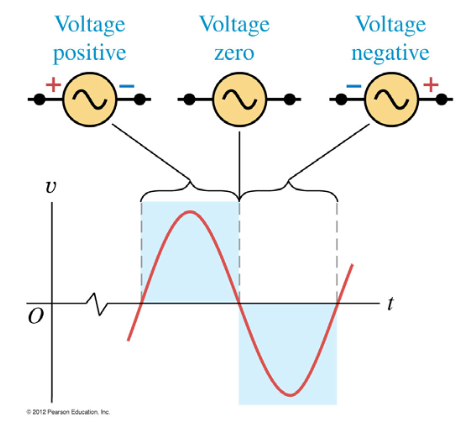
\includegraphics[width=0.90\textwidth]{./images/schematics/ac.png}\\
     \end{center}
  \end{column}
  \begin{column}{0.45\textwidth}
     This voltage will induce a current which, generally, is given by:
     \begin{equation*}
          I(t) = I_0 sin(\omega t + \phi)
     \end{equation*}
     where $\phi$ is the phase difference between the AC voltage and AC current.\\
     \vspace{0.2cm}
     {\small
       We will see that in an AC circuit that includes only resistors, the voltage and current have no phase difference ($\phi$ = 0)
       but in circuits with capacitors and inductors $\phi$ is  generally not 0.\\
     }
  \end{column}
\end{columns}

\end{frame}

%
%
%

\begin{frame}{Phasor diagrams}

\begin{columns}
  \begin{column}{0.45\textwidth}
    \begin{center}
       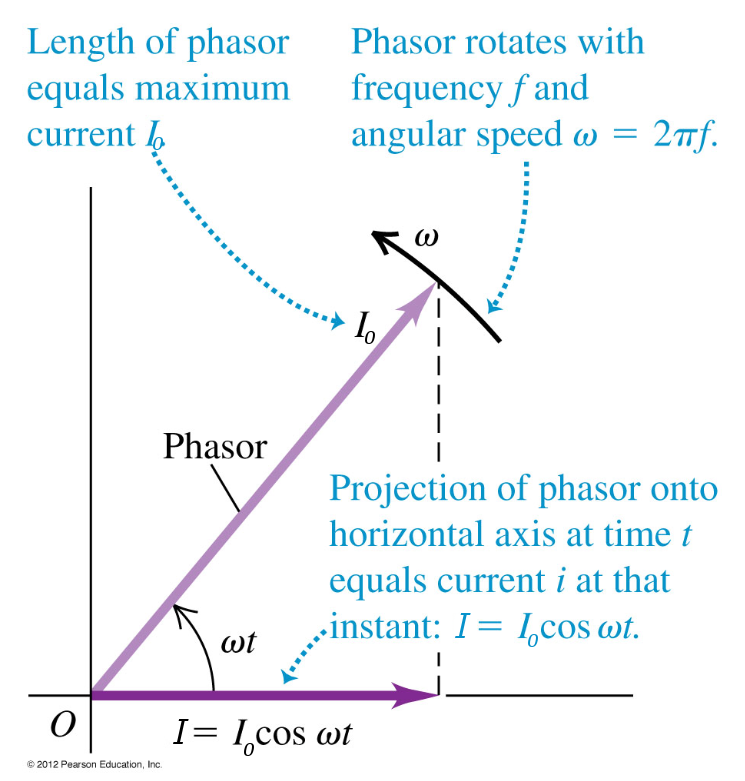
\includegraphics[width=0.96\textwidth]{./images/schematics/phasor_diagrams.png}\\
     \end{center}
  \end{column}
  \begin{column}{0.55\textwidth}
     It is convenient to represent the AC voltage V(t) and the AC current I(t) using {\em ``phasors''}.
     A phasor is a vector taken to be rotating counter-clockwisely with constant angular frequency $\omega$.
     \begin{itemize}
        \item The length of the phasor represents the magnitude of the quantity represented.
        \item The angle of the phasor represents its phase.
                  The usual reference for zero phase is taken to be the positive x-axis.
     \end{itemize}
  \end{column}
\end{columns}

\vspace{0.4cm}
Assume that the quantity represented is an AC current I:
At time t, the phase is $\omega  t$, and the projection of the phasor on the horizontal x axis
is $I_0 cos(\omega t)$, the value of I at time t (I(t)).

\end{frame}

%
%
%

\begin{frame}{AC generation: Simple alternator}

An {\bf alternator} is an electrical generator that converts mechanical energy to
electrical energy in the form of alternating current.

\begin{columns}
  \begin{column}{0.45\textwidth}
    \begin{center}
       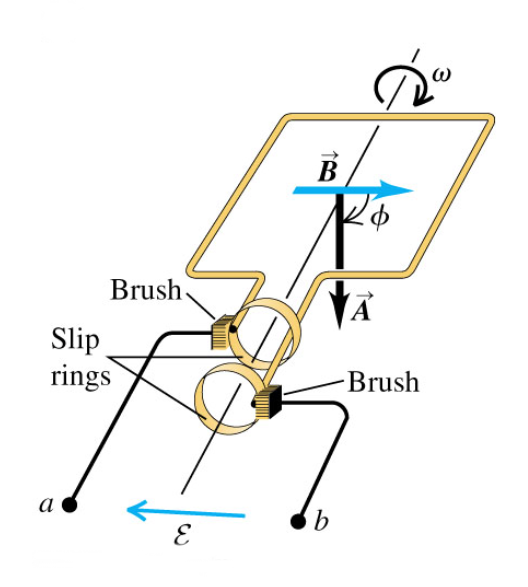
\includegraphics[width=0.98\textwidth]{./images/schematics/simple_alternator.png}\\
     \end{center}
  \end{column}
  \begin{column}{0.55\textwidth}
     \begin{itemize}
        \item A device that {\bf uses Faraday's law}:\\
                  A conductor moving relative to a magnetic field
                  develops an electromotive force (EMF) in it.
        \vspace{0.2cm}
        \item Typically, a {\bf rotating magnet (called the rotor)} turns within a {\bf stationary set of
                  conductors wound in coils (called the stator)}.
          \begin{itemize}
               \item the $\vec{B}$ field vector and the surface vector $\vec{S}$ rotate wrt each other.
         \end{itemize}
     \end{itemize}
  \end{column}
\end{columns}

\end{frame}

%
%
%

\begin{frame}{AC generation: Simple alternator}

\begin{columns}
  \begin{column}{0.25\textwidth}
    \begin{center}
       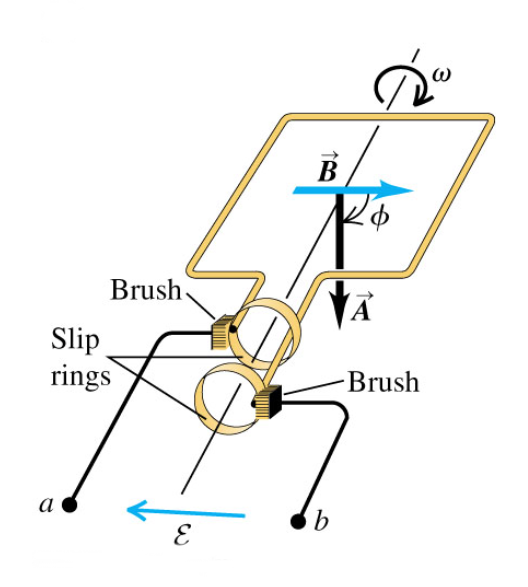
\includegraphics[width=0.95\textwidth]{./images/schematics/simple_alternator.png}\\
     \end{center}
  \end{column}
  \begin{column}{0.75\textwidth}
      Let’s call $\omega$ the angular frequency of that rotation.
      Assume that at t=0, the $\vec{B}$ and $\vec{S}$ vectors point towards the same direction.
      After time t, the opening angle $\phi$ between $\vec{B}$ and $\vec{S}$ will be:
      \begin{equation*}
          \phi = \omega t
      \end{equation*}
  \end{column}
\end{columns}

The magnetic flux through the conductor is:
\begin{equation*}
     \Phi_B = \int_{S} \vec{B} \cdot d\vec{S} = \vec{B} \cdot \vec{S} = B S cos\phi = B S cos(\omega t)
      \xRightarrow{{\Phi_B}_{0} = BS}
      {\color{magenta}
          \Phi_B =  {\Phi_B}_{0} cos(\omega t)
     }
\end{equation*}
The rate of change of the flux gives us the EMF:
\begin{equation*}
     \mathcal{E} = - \frac{d}{dt} \Phi_B = - \frac{d}{dt} \Big(  B S cos(\omega t) \Big) = \omega B S  sin(\omega t)
     \xRightarrow{\mathcal{E}_0 =  \omega B S}
      {\color{magenta}
        \mathcal{E} = \mathcal{E}_0 sin(\omega t)
      }
\end{equation*}

\end{frame}


%
%
%

\begin{frame}{AC generation: Simple alternator}

The rotating $\vec{B}$ field {\bf induces an AC voltage} in the stator windings:
\begin{equation*}
     \Phi_B = {\Phi_B}_{0}  cos(\omega t) \;\;\;\;\; \rightarrow \;\;\;\;\; \mathcal{E} = \mathcal{E}_0 sin(\omega t)
\end{equation*}

\begin{center}
    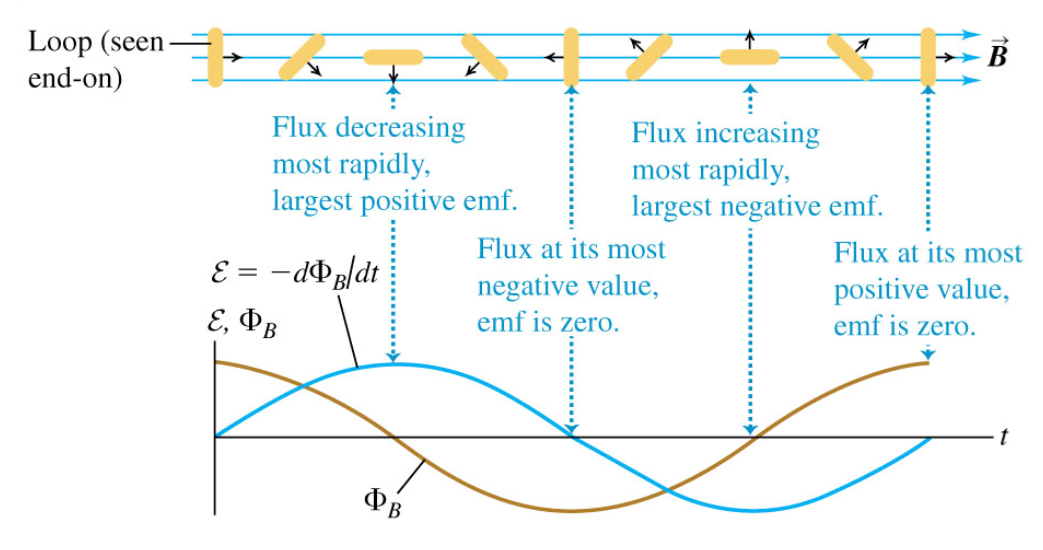
\includegraphics[width=0.80\textwidth]{./images/schematics/simple_alternator_operation.png}\\
\end{center}

Notice that there is a phase of $\pi$/2 between the flux and the voltage:
\begin{itemize}
   \item $\displaystyle cos(\omega t) = sin(\omega t + \frac{\pi}{2})$ $\rightarrow$ The flux leads
\end{itemize}


\end{frame}

%
%
%


\begin{frame}{Forced (or driven) oscillations}

Before, we studied {\bf undamped LC} and {\bf damped RLC} circuits.
\begin{itemize}
  \item They oscillated at angular frequency $\displaystyle \omega_0 = \frac{1}{\sqrt{LC}}$
  \item Such oscillations are {\bf free oscillations}
  \item $\displaystyle \omega_0$ is the circuit's {\bf natural angular frequency}.
\end{itemize}

\begin{columns}
  \begin{column}{0.50\textwidth}
     \begin{center}
         \begin{circuitikz} [scale=0.8]
            \draw
                 (0,0) to[battery=$\varepsilon$] (0,2) to[short, -o] (0.75, 2.0);
             \draw[very thick]
                  (0.78,2.0)--(1.18,2.3);
             \draw
                  (1.25, 2.0) to [short, o-] (2,2) to[C=$C$] (2,0)--(0,0);
              \draw
                  (2,2)--(4,2) to[L=$L$,i=$I$] (4,0) -- (2,0);
         \end{circuitikz}
     \end{center}
  \end{column}
  \begin{column}{0.50\textwidth}
     \begin{center}
         \begin{circuitikz} [scale=0.8]
            \draw
                 (0,0) to[battery=$\varepsilon$] (0,2) to[short, -o] (0.75, 2.0);
             \draw[very thick]
                  (0.78,2.0)--(1.18,2.3);
             \draw
                  (1.25, 2.0) to [short, o-] (2,2) to[C=$C$] (2,0)--(0,0);
              \draw
                  (2,2) to[R=$R$]  (4,2) to[L=$L$,i=$I$] (4,0) -- (2,0);
         \end{circuitikz}
     \end{center}
  \end{column}
\end{columns}

\vspace{0.2cm}

In this lecture we will consider {\bf forced (or driven) oscillations}.\\

\vspace{0.3cm}
{\small
When the RLC circuit is connected to an alternating EMF
$\mathcal{E} = \mathcal{E}_0 sin(\omega t)$, the oscillations of
charge, voltage and current can occur at the driving frequency $\omega$.
}
\end{frame}

%
%
%


\begin{frame}{Resistor, Capacitor and Inductor in an AC circuit}

We will study the {\bf forced (or driven) oscillation} of the RLC circuit.\\

\vspace{0.2cm}

First, we will study the behaviour of different simple AC circuits:\\

\vspace{0.2cm}

\begin{columns}
  \begin{column}{0.33\textwidth}
    \begin{center}
         \begin{circuitikz}
            \draw
                 (0,0) to[sinusoidal voltage source=$\varepsilon$] (0,2) -- (2,2)
                         to[R=$R$, i=$I$, v=$V_R$] (2,0) -- (0,0);
         \end{circuitikz}
          {\small \color{magenta} Purely resistive load}
     \end{center}
  \end{column}
  \begin{column}{0.33\textwidth}
    \begin{center}
         \begin{circuitikz}
            \draw
                 (0,0) to[sinusoidal voltage source=$\varepsilon$] (0,2) -- (2,2)
                         to[C=$C$, i=$I$, v=$V_C$] (2,0) -- (0,0);
         \end{circuitikz}
         {\small \color{magenta} Purely capacitive load}
     \end{center}
  \end{column}
  \begin{column}{0.33\textwidth}
    \begin{center}
         \begin{circuitikz}
            \draw
                 (0,0) to[sinusoidal voltage source=$\varepsilon$] (0,2) -- (2,2)
                         to[L=$C$, i=$I$, v=$V_L$] (2,0) -- (0,0);
         \end{circuitikz}
          {\small \color{magenta} Purely inductive load}
     \end{center}
  \end{column}
\end{columns}

\vspace{0.6cm}

In particular we will study what is the current $I(t)$ and the voltage $V_i(t)$ across the two ends of the
resistor, capacitor and inductor (i = R,L,C) connected in the circuit with an AC voltage
$\displaystyle \mathcal{E} = \mathcal{E}_0 sin(\omega t)$.

\end{frame}


%
%
%


\begin{frame}{Resistor in an AC circuit}

\begin{columns}
  \begin{column}{0.35\textwidth}
    \begin{center}
         \begin{circuitikz}
            \draw
                 (0,0) to[sinusoidal voltage source=$\varepsilon$] (0,2) -- (2,2)
                         to[R=$R$, i=$I$, v=$V_R$] (2,0) -- (0,0);
         \end{circuitikz}
     \end{center}
  \end{column}
  \begin{column}{0.65\textwidth}
       $V_R(t)$ is given by Kirchoff's voltage rule:
       \begin{equation*}
           \mathcal{E}(t) = V_R(t) \Rightarrow
            V_R(t) = \mathcal{E}_0 sin(\omega t) \Rightarrow
       \end{equation*}
       \begin{equation*}
            {\color{magenta}
                 V_R(t) = {V_R}_0 sin(\omega t)
            }
       \end{equation*}
       where ${V_R}_0 = \mathcal{E}_0$.
  \end{column}
\end{columns}

\vspace{0.4cm}

The current $I(t)$ is given by:
\begin{equation*}
      V_R(t) = I(t) R \Rightarrow I(t) = \frac{V_R(t)}{R} \Rightarrow  I(t) = \frac{V_0}{R} sin(\omega t) \Rightarrow
      {\color{magenta}
                 I(t) = I_0 sin(\omega t)
      }
\end{equation*}
where $I_0 = {V_R}_0/R$.\\

\end{frame}

%
%
%

\begin{frame}{Resistor in an AC circuit}

\begin{center}
{\scriptsize
\begin{equation*}
   {\color{magenta}  I(t) = I_0 sin(\omega t) } \; and \;
   {\color{magenta}  V_R(t) = {V_R}_0 sin(\omega t)} \;
   where \; I_0 = \frac{{V_R}_0}{R}, \; and \; {V_R}_0 = \mathcal{E}_0
\end{equation*}
}
{\color{magenta}
  {\bf Current and voltage are always in phase.}
}
\end{center}

\begin{columns}
  \begin{column}{0.50\textwidth}
    \begin{center}
       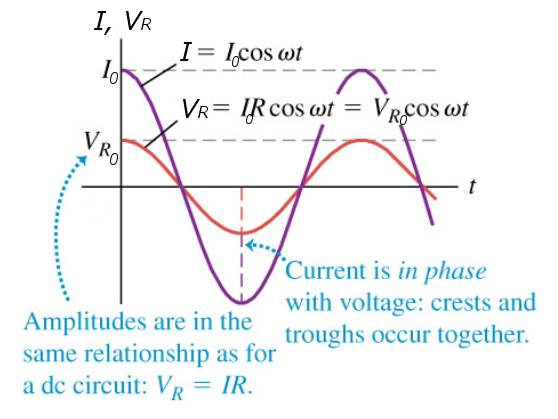
\includegraphics[width=0.98\textwidth]{./images/schematics/ac_resistor_graph.png}\\
     \end{center}
  \end{column}
  \begin{column}{0.50\textwidth}
    \begin{center}
       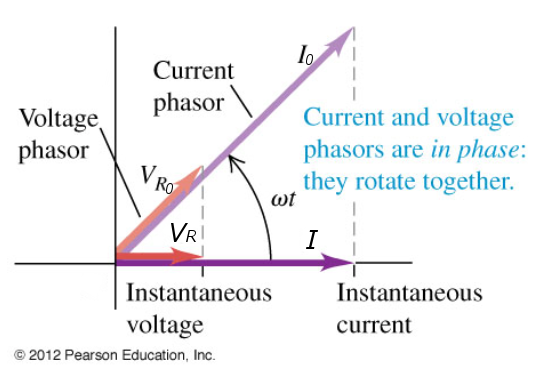
\includegraphics[width=0.98\textwidth]{./images/schematics/ac_resistor_phasor.png}\\
     \end{center}
  \end{column}
\end{columns}

\end{frame}

%
%
%

\begin{frame}{Capacitor in an AC circuit}

\begin{columns}
  \begin{column}{0.35\textwidth}
    \begin{center}
         \begin{circuitikz}
            \draw
                 (0,0) to[sinusoidal voltage source=$\varepsilon$] (0,2) -- (2,2)
                         to[C=$C$, i=$I$, v=$V_C$] (2,0) -- (0,0);
         \end{circuitikz}
     \end{center}
  \end{column}
  \begin{column}{0.65\textwidth}
        $V_C(t)$ is given by Kirchoff's voltage rule:
        \begin{equation*}
           \mathcal{E}(t) = V_C(t) \Rightarrow
            {\color{magenta}
                 V_C(t) = {V_C}_0 sin(\omega t)
            }
        \end{equation*}
        where ${V_C}_0 = \mathcal{E}_0$.
  \end{column}
\end{columns}

\vspace{0.2cm}

The current $I(t)$ is calculated as follows:
\begin{equation*}
     V_C(t) = \frac{Q(t)}{C} \Rightarrow Q(t) = C  V_C(t) \Rightarrow   Q(t) = C {V_C}_0 sin(\omega t) \xRightarrow{I = dQ/dt}
\end{equation*}
\begin{equation*}
      I(t) =\omega C {V_C}_0 cos(\omega t) \Rightarrow
      \xRightarrow{cos\theta = sin\Big( \theta + \frac{\pi}{2} \Big)}
      {\color{magenta}
                 I(t) = I_0 sin\Big(\omega t + \frac{\pi}{2} \Big)
      }
\end{equation*}
where $\displaystyle I_0 = \omega C {V_C}_0 = \frac{{V_C}_0}{X_C}$.\\
\vspace{0.1cm}
The quantity {\color{magenta}
  $\displaystyle X_C = \frac{1}{\omega C}$ is the so-called {\bf capacitive reactance}
}.

\end{frame}

%
%
%

\begin{frame}{Capacitor in an AC circuit}

\begin{center}
{\scriptsize
\begin{equation*}
   {\color{magenta}  I(t) = I_0 sin \Big(\omega t + \frac{\pi}{2} \Big) } \; and \;
   {\color{magenta}  V_C(t) = {V_C}_0 sin(\omega t)} \;
   where \; I_0 = \frac{{V_C}_0}{X_C}, \; {V_C}_0 = \mathcal{E}_0, \; and \; X_C = \frac{1}{\omega C}
\end{equation*}
}
{\color{magenta}
  {\bf Current leads voltage by $\pi/2$.}
}
\end{center}

\begin{columns}
  \begin{column}{0.50\textwidth}
    \begin{center}
       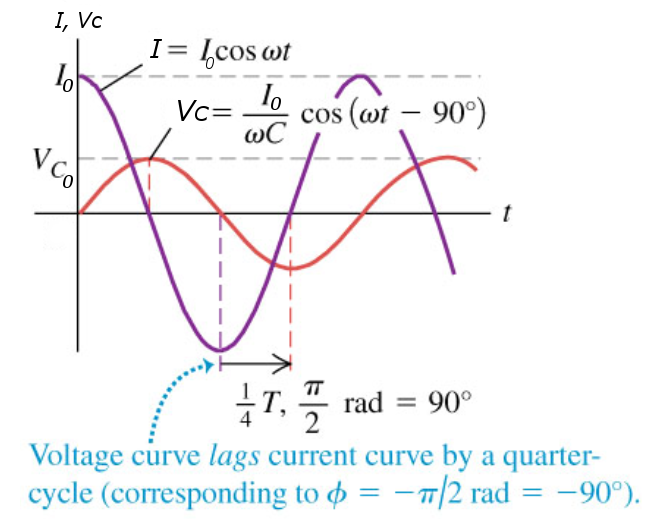
\includegraphics[width=0.98\textwidth]{./images/schematics/ac_capacitor_graph.png}\\
     \end{center}
  \end{column}
  \begin{column}{0.50\textwidth}
    \begin{center}
       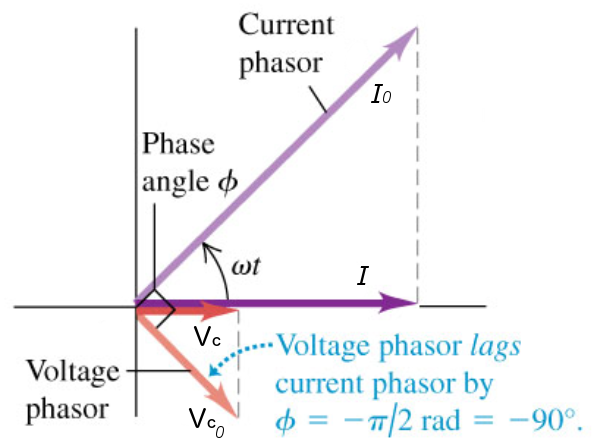
\includegraphics[width=0.98\textwidth]{./images/schematics/ac_capacitor_phasor.png}\\
     \end{center}
  \end{column}
\end{columns}

\end{frame}


%
%
%

\begin{frame}{Inductor in an AC circuit}

\begin{columns}
  \begin{column}{0.35\textwidth}
    \begin{center}
         \begin{circuitikz}
            \draw
                 (0,0) to[sinusoidal voltage source=$\varepsilon$] (0,2) -- (2,2)
                         to[L=$C$, i=$I$, v=$V_L$] (2,0) -- (0,0);
         \end{circuitikz}
     \end{center}
  \end{column}
  \begin{column}{0.65\textwidth}
        $V_L(t)$ is given by Kirchoff's voltage rule:
        \begin{equation*}
           \mathcal{E}(t) - V_L(t) = 0 \Rightarrow
            {\color{magenta}
                 V_L(t) = {V_L}_0 sin(\omega t)
            }
        \end{equation*}
        where ${V_L}_0 = \mathcal{E}_0$.
  \end{column}
\end{columns}

\vspace{0.2cm}

The current $I(t)$ is calculated as follows:
\begin{equation*}
     V_L(t) = L \frac{dI(t)}{dt} \Rightarrow
     I(t) = \frac{1}{L} \int V_L(t) dt \Rightarrow
     I(t) =\frac{{V_L}_0}{L}  \int sin(\omega t) dt \Rightarrow
\end{equation*}
\begin{equation*}
      I(t) =- \frac{{V_L}_0}{\omega L} cos(\omega t)
      \xRightarrow{-cos\theta = sin\Big( \theta - \frac{\pi}{2} \Big)}
      {\color{magenta}
             I(t) = I_0 sin\Big(\omega t - \frac{\pi}{2} \Big)
      }
\end{equation*}
where $\displaystyle I_0 =\frac{{V_L}_0}{\omega L} = \frac{{V_L}_0}{X_L}$.\\
\vspace{0.2cm}
The quantity {\color{magenta}
  $\displaystyle X_L = \omega L$ is the so-called {\bf inductive reactance}
}.


\end{frame}

%
%
%

\begin{frame}{Inductor in an AC circuit}

\begin{center}
{\scriptsize
\begin{equation*}
   {\color{magenta}  I(t) = I_0 sin \Big(\omega t - \frac{\pi}{2} \Big) } \; and \;
   {\color{magenta}  V_L(t) = {V_L}_0 sin(\omega t)} \;
   where \; I_0 = \frac{{V_L}_0}{X_L}, \; {V_L}_0 = \mathcal{E}_0 \; and \; X_L = \omega L
\end{equation*}
}
{\color{magenta}
  {\bf Voltage leads current by $\pi/2$.}
}
\end{center}

\begin{columns}
  \begin{column}{0.50\textwidth}
    \begin{center}
       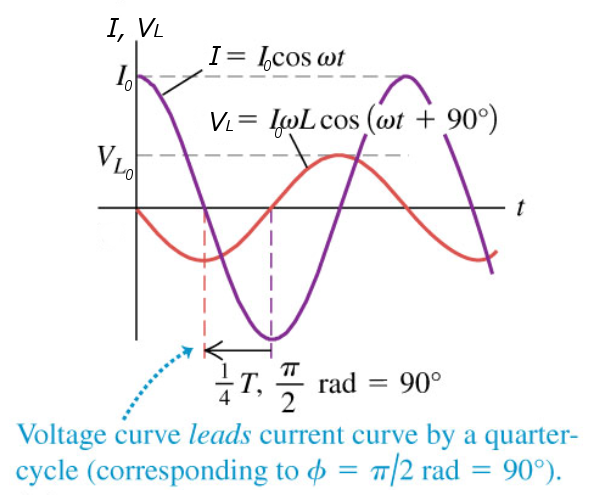
\includegraphics[width=0.90\textwidth]{./images/schematics/ac_inductor_graph.png}\\
     \end{center}
  \end{column}
  \begin{column}{0.50\textwidth}
    \begin{center}
       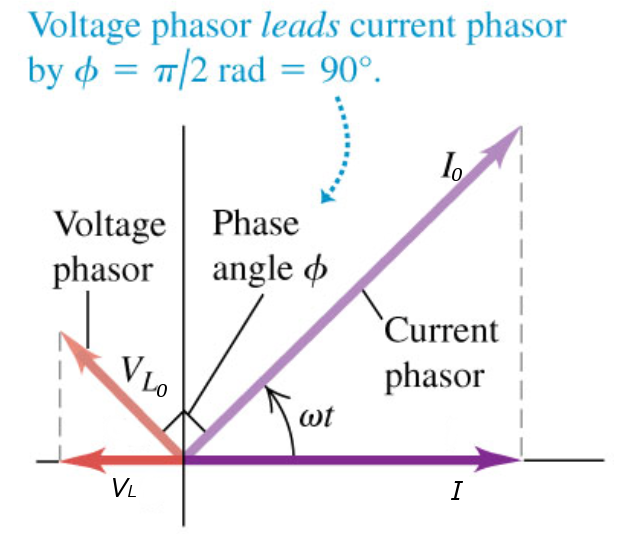
\includegraphics[width=0.90\textwidth]{./images/schematics/ac_inductor_phasor.png}\\
     \end{center}
  \end{column}
\end{columns}

\end{frame}

%
%
%

\begin{frame}{Summary: R, L, C elements in an AC circuit}

\begin{columns}
  \begin{column}{0.60\textwidth}
    \begin{center}
       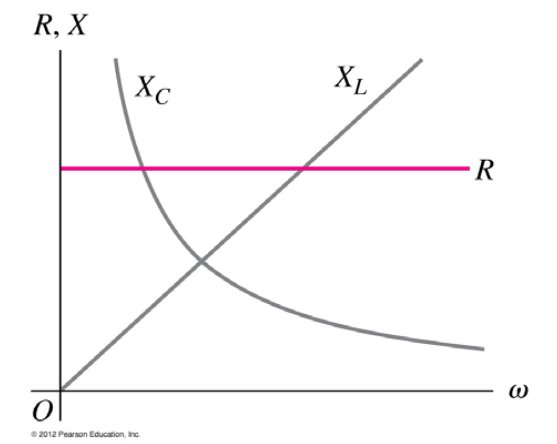
\includegraphics[width=0.85\textwidth]{./images/schematics/reactance_freq_dependence.png}\\
     \end{center}
  \end{column}
  \begin{column}{0.40\textwidth}
        {\bf Resistance / Reactance}\\
        \vspace{0.2cm}
        \begin{itemize}
           \item Resistor: R
           \item Capacitor: $\displaystyle X_C = \frac{1}{\omega C}$
           \item Inductor: $\displaystyle X_L = \omega L$
        \end{itemize}
  \end{column}
\end{columns}

\begin{itemize}
{\small
\item Capacitance causes poor response to low frequencies.
\item Inductance causes poor response to high frequencies.
\item For an RLC circuit, the response is maximised around some intermediate resonant frequency.
}
\end{itemize}

\end{frame}

%
%
%

\begin{frame}{Summary: R, L, C elements in an AC circuit}

\begin{equation*}
{\color{magenta}
     V_i(t) = {V_i}_0 sin(\omega t) \;\;\; [i=R,L,C]
     \;\;\;\; and \;\;\;\;
     I(t) = \frac{{V_i}_0}{ {\color{blue}X}} sin(\omega t + {\color{blue}\phi})
}
\end{equation*}

\setlength{\extrarowheight}{12pt}
\setlength{\arraycolsep}{5pt}

 \begin{center}
 {

  \begin{table}[H]
    \begin{tabular}{|c|c|c|c|}
      \hline
        {\bf Element} & {\bf Resistance/} & {\bf Current} & {\bf Frequency} \\
                      & {\bf Reactance}   & {\bf phase}    & {\bf response} \\
      \hline
        Resistor  &
            $\displaystyle R$  &
            $\displaystyle \phi = 0$  &
            DC, AC: all frequencies \\
        Capacitor &
            $\displaystyle X_C = \frac{1}{\omega C}$  &
            $\displaystyle \phi = +\frac{\pi}{2}$  &
            no DC, AC: high-pass filter \\
        Inductor  &
            $\displaystyle X_L = \omega L$  &
            $\displaystyle \phi = -\frac{\pi}{2}$   &
            DC, AC: low-pass filter \\
      \hline
    \end{tabular}
  \end{table}

 }
 \end{center}

\end{frame}


%
%
%

\begin{frame}{Application: Audio crossover}

{ \scriptsize
Audio crossovers are a class of electronic filter used in audio applications.
Most individual loudspeaker drivers are incapable of covering the entire audio spectrum from low frequencies
to high frequencies with acceptable relative volume and absence of distortion so most hi-fi speaker systems
use a combination of multiple loudspeaker drivers, each catering to a different frequency band.
Crossovers split the audio signal into separate frequency bands that can be separately routed to loudspeakers
optimized for those bands [from Wikipedia].\\
}

\begin{center}
     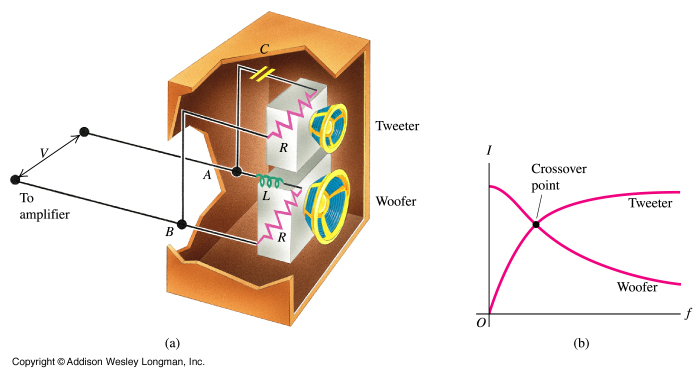
\includegraphics[width=0.70\textwidth]{./images/schematics/crossover_network_in_speaker.jpg}\\
\end{center}

The crossover frequency is determined by $X_L$ = $X_C$

\end{frame}


%
%
%

\begin{frame}{The RLC series AC circuit}

    Now are now ready to study a circuit with a resistor, inductor and capacitor connected in series
    and connected to an external alternating EMF.\\
    \vspace{0.2cm}

    \begin{center}
         \begin{circuitikz} [scale=1.60]
            \draw
                 (0,0) to[sinusoidal voltage source=$\varepsilon$] (0,2)
                         to[R=$R$, i=$I$, v=$V_R$] (2,2)
                         to[L=$L$,  i=$I$, v=$V_L$] (2,0)
                         to[C=$C$, i=$I$, v=$V_C$] (0,0);
         \end{circuitikz}
     \end{center}

\end{frame}

%
%
%

\begin{frame}{The RLC series AC circuit}


The {\bf current is common}:
\begin{equation*}
    I_R(t) =  I_L(t) = I_C(t) = I(t)
\end{equation*}

\vspace{0.2cm}
Assume: $\displaystyle I(t) = I_0 sin(\omega t)$.\\

\begin{columns}
  \begin{column}{0.40\textwidth}
    \begin{center}
        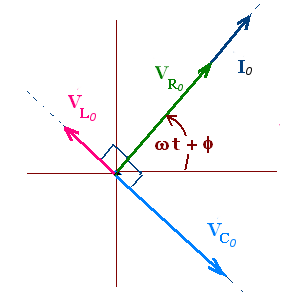
\includegraphics[width=0.99\textwidth]{./images/schematics/ac_rlc_phasor_diagram_01.png}\\
     \end{center}
  \end{column}
  \begin{column}{0.60\textwidth}
      The voltages across the R, L, C elements can be written as:
      \begin{equation*}
          V_R(t) = {\color{blue} I_0 R} sin({\color{magenta} \omega t}); \;\;
      \end{equation*}
      \begin{equation*}
          V_L(t) = {\color{blue} I_0 X_L} sin\Big({\color{magenta} \omega t + \frac{\pi}{2} } \Big); \;\;
      \end{equation*}
      \begin{equation*}
          V_C(t) = {\color{blue} I_0 X_C} sin\Big({\color{magenta} \omega t - \frac{\pi}{2} } \Big)
      \end{equation*}
  \end{column}
\end{columns}

\end{frame}

%
%
%

\begin{frame}{The RLC series AC circuit}

\begin{center}
   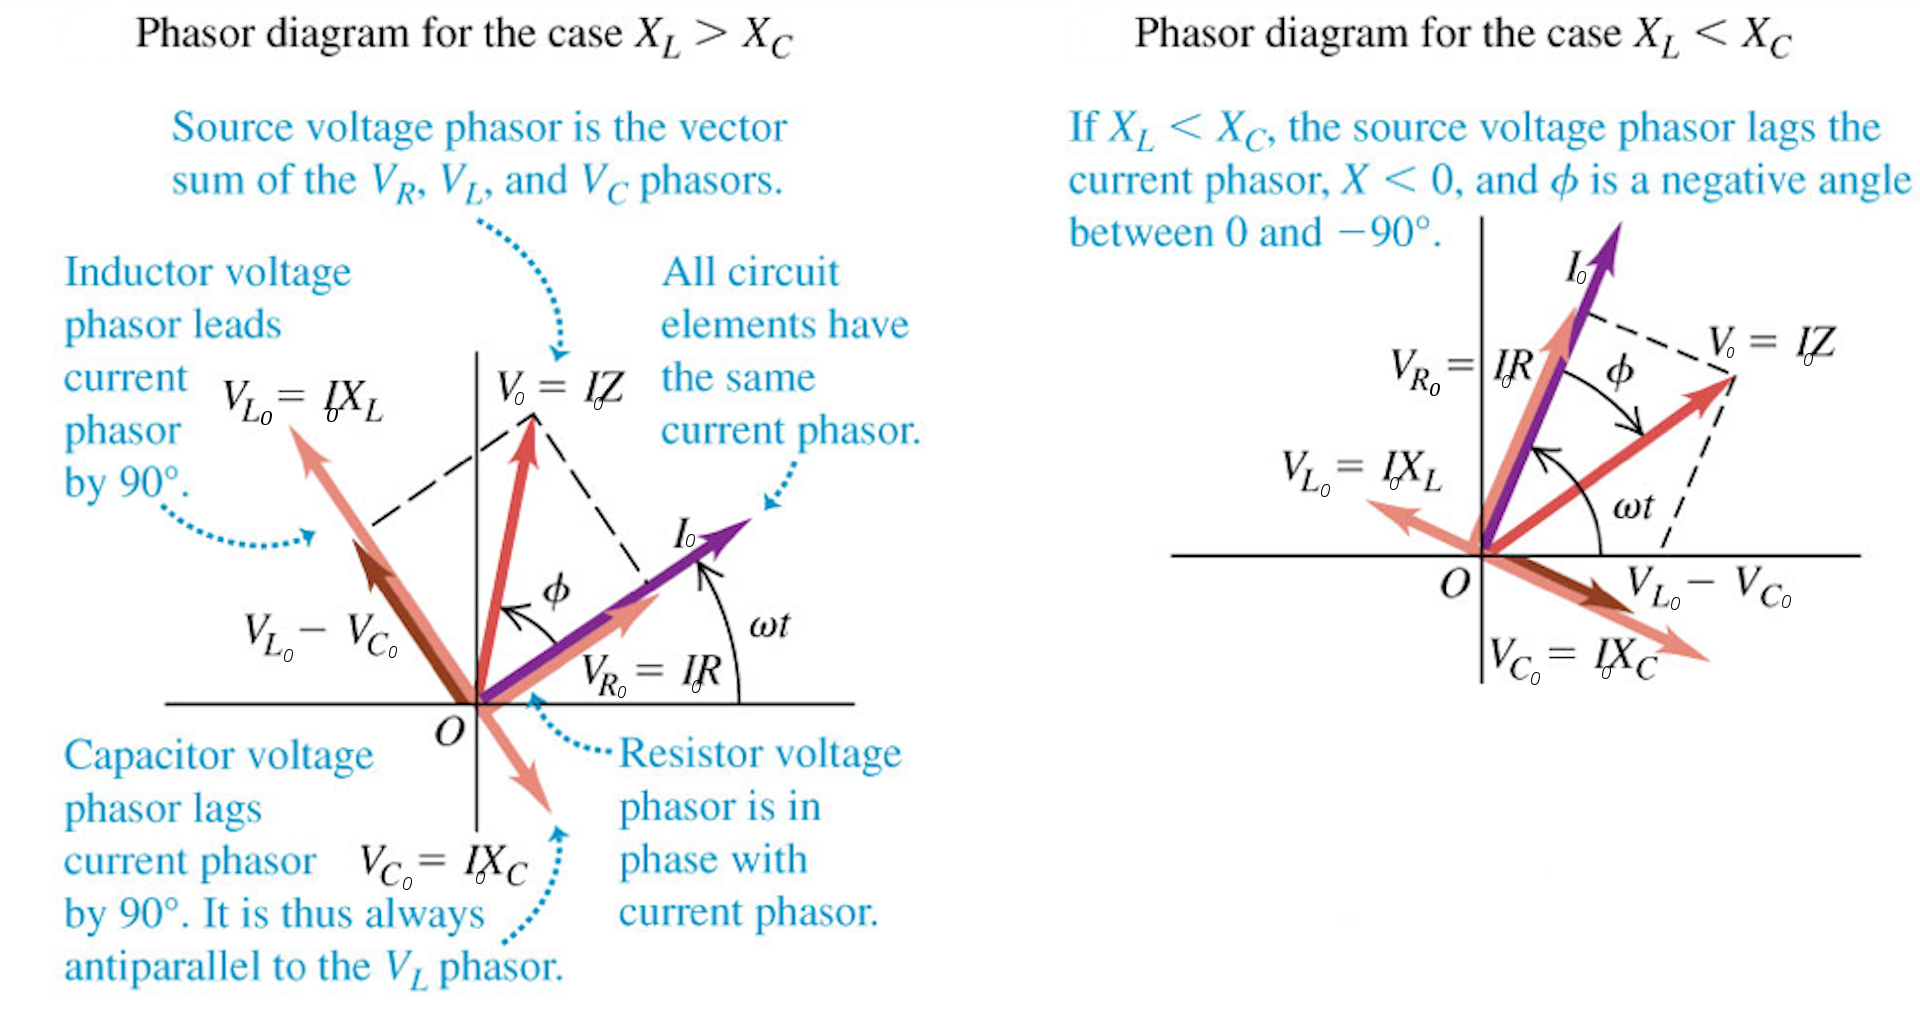
\includegraphics[width=0.99\textwidth]{./images/schematics/ac_rlc_phasor_diagram_02.png}\\
\end{center}


\end{frame}

%
%
%

\begin{frame}{The RLC series AC circuit}

Kirchoff's voltage rule is valid at all times t as the phasors rotate together:
\begin{equation*}
    \mathcal{E}(t) = V_R(t) + V_L(t)  + V_C(t)
\end{equation*}

Because the phasors representing the voltages in the inductor and the capacitor have opposite directions
and they are perpendicular to the phasor representing the voltage in the resistor:
\begin{equation*}
    \mathcal{E}_0^2 = {V_R}_0^2 + \Big( {V_L}_0 - {V_C}_0 \Big)^2  \Rightarrow
\end{equation*}

\begin{equation*}
    \mathcal{E}_0^2 = I_0^2 R^2 + \Big( I_0 X_L - I_0 X_C \Big)^2 = I_0^2 \Big\{ R^2 + \Big( X_L - X_C \Big)^2  \Big\} \Rightarrow
\end{equation*}

\begin{equation*}
        I_0 = \frac{\mathcal{E}_0}{\sqrt{R^2 + \Big( X_L - X_C \Big)^2}} =
                 \frac{\mathcal{E}_0}{\sqrt{R^2 + \Big( \omega L - \frac{1}{\omega C} \Big)^2}} =
                 \frac{\mathcal{E}_0}{Z}
\end{equation*}

where {\color{magenta} $\displaystyle Z = \sqrt{R^2 + \Big( \omega L - \frac{1}{\omega C} \Big)^2}$}
is the {\bf impedance} of the RLC circuit.\\

\end{frame}

%
%
%

\begin{frame}{The RLC series AC circuit}

The value of $I_0$ depends on the difference between
$\displaystyle \omega L$ and $\displaystyle \frac{1}{\omega C}$
(i.e. the difference between $X_L$ and $X_R$)
\begin{itemize}
  \item Doesn't matter which one is greater as the difference is squared.
\end{itemize}

\begin{equation*}
{\color{magenta}
        I_0 = \frac{\mathcal{E}_0}{Z} =
                 \frac{\mathcal{E}_0}{\sqrt{R^2 + \Big( \omega L - \frac{1}{\omega C} \Big)^2}}
}
\end{equation*}

But which one is greater determines the phase $\phi$
by which the voltage leads the current:
\begin{equation*}
     tan\phi = \frac{V_L - V_C}{V_R} \Rightarrow {\color{magenta}  tan\phi = \frac{X_L - X_C}{R} }
\end{equation*}

\begin{itemize}
  \item  {\color{magenta}  $X_L > X_C$}: The circuit is {\bf more inductive than capacitive}.
      \begin{itemize}
         \item The current trails behind the voltage (voltage leads).
      \end{itemize}
  \item  {\color{magenta}  $X_L < X_C$}: The circuit is {\bf more capacitive then inductive}.
      \begin{itemize}
         \item The current leads.
      \end{itemize}
  \item  {\color{magenta}  $X_L = X_C$}: ?
\end{itemize}


\end{frame}

%
%
%

\begin{frame}{The RLC series AC circuit: Resonance condition}

If $X_L = X_C$, the circuit is {\bf in resonance}.

\begin{columns}
  \begin{column}{0.60\textwidth}
    \begin{center}
        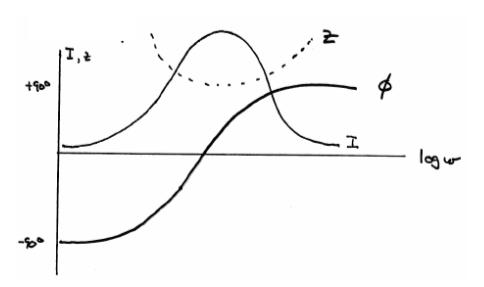
\includegraphics[width=0.99\textwidth]{./images/schematics/ac_rlc_resonance.png}\\
     \end{center}
  \end{column}
  \begin{column}{0.40\textwidth}
    At resonance, we have
    \begin{itemize}
       \item minimum impedance,
       \item maximal current, and
       \item current in phase with voltage in ($\phi=0$)
     \end{itemize}
  \end{column}
\end{columns}

\begin{equation*}
  X_L = X_C \Rightarrow \omega L - \frac{1}{\omega C} = 0 \Rightarrow \omega = \frac{1}{\sqrt{LC}}
\end{equation*}

The resonance happens when the {\bf driving angular frequency matches the natural angular frequency}.

\end{frame}

%
%
%

\begin{frame}{The RLC series AC circuit: Resonance condition}

Resonant circuits are used to {\bf respond selectively to signals of a given
frequency} while {\bf discriminating against signals of different frequencies}.\\

\vspace{0.2cm}

An example of the application of resonant circuits: selection of AM radio stations.

\begin{columns}
  \begin{column}{0.50\textwidth}
    \begin{center}
     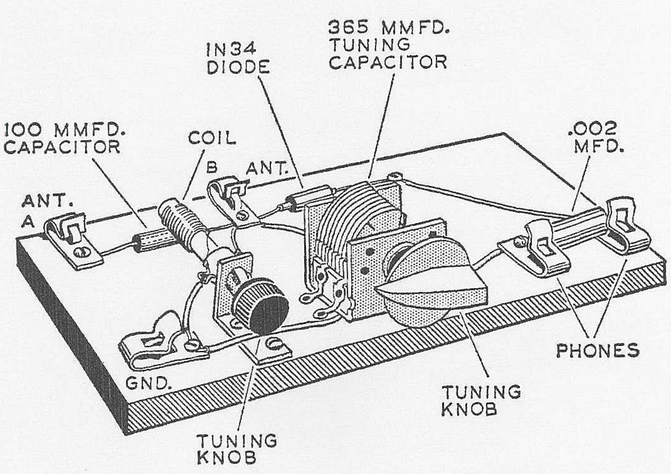
\includegraphics[width=0.99\textwidth]{./images/schematics/am_radio.png}\\
     \end{center}
  \end{column}
  \begin{column}{0.50\textwidth}
    \begin{center}
     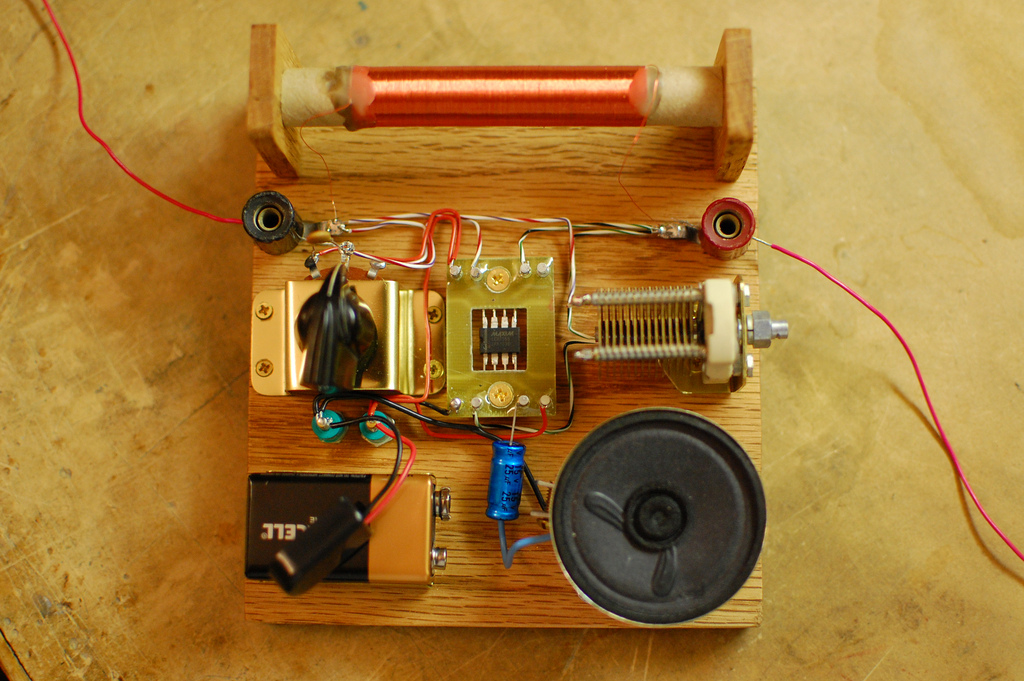
\includegraphics[width=0.99\textwidth]{./images/photos/am_radio.jpg}\\
     \end{center}
  \end{column}
\end{columns}

\end{frame}

%
%
%

\begin{frame}{Power in the RLC series circuit}

\begin{itemize}

\item
Average power dissipated on resistor:
\begin{equation*}
      P_{avg} = \frac{1}{T} \int_{0}^{T} V_R(t) I(t) = \frac{1}{2} {V_R}_0 I_0 = {V_R}_{rms} I_{rms} = I_{rms}^2 R = \frac{{V_R}_{rms}^2}{R}
\end{equation*}

\item
The inductor stores and releases energy periodically in the $\vec{B}$ field.

\item
The capacitor stores and releases energy periodically in the $\vec{E}$ field.

\end{itemize}

\vspace{0.2cm}

Average power provided by a generator:
\begin{equation*}
      P_{avg} = \frac{1}{2} V_0 I_0 cos\phi = V_{rms} I_{rms} cos\phi
\end{equation*}

\noindent\rule{2cm}{0.4pt}\\
{ \scriptsize
  Note that $\displaystyle \int_{0}^{2\pi} sin^2x dx = \frac{1}{2}$ leads to $\displaystyle I_{rms} = \frac{I_0}{\sqrt{2}}$
  and $\displaystyle {V_R}_{rms} = \frac{V_0}{\sqrt{2}}$
}

\end{frame}

%
%
%

\begin{frame}{Power in the RLC series circuit}

\begin{center}
   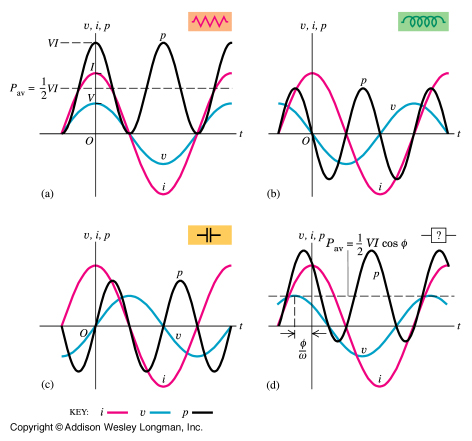
\includegraphics[width=0.70\textwidth]{./images/schematics/ac_rlc_power.png}\\
\end{center}

\end{frame}

%
%
%

\begin{frame}{Lecture \thislecture - What to remember}

{\small

When the RLC circuit is connected to an alternating EMF
$\mathcal{E} = \mathcal{E}_0 sin(\omega t)$, the oscillations of
charge, voltage and current can occur at the driving frequency $\omega$.\\

\vspace{0.2cm}

\begin{equation*}
{\color{magenta}
     V_i(t) = {V_i}_0 sin(\omega t) \;\;\; [i=R,L,C]
     \;\;\;\; and \;\;\;\;
     I(t) = \frac{{V_i}_0}{ {\color{blue}X}} sin(\omega t + {\color{blue}\phi})
}
\end{equation*}

 \begin{center}
 {
  \begin{table}[H]
    \begin{tabular}{|c|c|c|c|}
      \hline
        {\bf Element} & {\bf Resistance/} & {\bf Current} & {\bf Frequency} \\
                      & {\bf Reactance}   & {\bf phase}    & {\bf response} \\
      \hline
        Resistor   &
             $\displaystyle R$   &
             $\displaystyle \phi = 0$  &
             DC, AC: all frequencies \\
        Capacitor  &
             $\displaystyle X_C = \frac{1}{\omega C}$   &
             $\displaystyle \phi = +\frac{\pi}{2}$   &
             no DC, AC: high-pass filter \\
        Inductor   &
             $\displaystyle X_L = \omega L$  &
             $\displaystyle \phi = -\frac{\pi}{2}$  &
             DC, AC: low-pass filter \\
      \hline
    \end{tabular}
  \end{table}

 }
 \end{center}

In an RLC circuit:
\begin{equation*}
{\color{magenta}
        I_0 = \frac{\mathcal{E}_0}{Z} =
                 \frac{\mathcal{E}_0}{\sqrt{R^2 + \Big( \omega L - \frac{1}{\omega C} \Big)^2}}
}
\end{equation*}
where Z is the impedance of the circuit.
}
\end{frame}

% ------------------------------------------------------------------------------
% ------------------------------------------------------------------------------

%
% What to remember
%

\renewcommand{\lecturesummarytitle}{Main points to remember }

\renewcommand{\summarizedlecture}{12 }

%
%
%

\begin{frame}{Lecture \summarizedlecture - \lecturesummarytitle}

{\small

In an RLC circuit, the phase $\phi$ by which the voltage leads the current is given by:
\begin{equation*}
     tan\phi = \frac{V_L - V_C}{V_R} \Rightarrow {\color{magenta}  tan\phi = \frac{X_L - X_C}{R} }
\end{equation*}

\begin{itemize}
  \item  {\color{magenta}  $X_L > X_C$}: The circuit is {\bf more inductive than capacitive} (voltage leads).
  \item  {\color{magenta}  $X_L < X_C$}: The circuit is {\bf more capacitive then inductive} (current leads).
  \item  {\color{magenta}  $X_L = X_C$}: the circuit is {\bf in resonance}
      \begin{itemize}
       {\scriptsize
          \item min. impedance,  max. current, and current in phase with voltage in ($\phi=0$)
       }
      \end{itemize}
\end{itemize}

The resonance happens when the {\bf driving angular frequency matches the natural angular frequency}:
\begin{equation*}
  X_L = X_C \Rightarrow \omega = \frac{1}{\sqrt{LC}}
\end{equation*}

}
\end{frame}

